\subsection{Дополнительный эксперимент 2: мультиактивная проверка на crypto-news}

Дополнительный эксперимент 1 показал, что для AAPL добавление FinBERT embeddings к расширенному рыночному baseline не даёт устойчивого улучшения. Поэтому был проведён дополнительный эксперимент RUN 05, цель которого состоит в проверке того, сохраняется ли этот вывод при переходе к другому классу активов, другому источнику текстов и нескольким горизонтам прогноза.

В RUN 05 использовались новости из датасета \texttt{crypto-news}. Для получения ценовых данных новости были объединены с дневными OHLCV-данными Binance. Это позволило не зависеть от \texttt{yfinance} и построить единый датасет для криптоактивов. В итоговую проверку вошли BNB, BTC и SOL на горизонтах 1, 3 и 7 дней. Целевая переменная задаётся как

\[
y_{t,h}=\mathbf{1}\{Close_{t+h}>Close_t\},
\]

где $h \in \{1,3,7\}$ --- горизонт прогноза в днях.

В отличие от дополнительного эксперимента 1, где использовался полный 768-мерный FinBERT embedding, в RUN 05 использовались более компактные FinBERT-derived признаки: вероятности sentiment-классов, sentiment-score, модуль sentiment-score и text-meta признаки. Такой вариант более устойчив для небольших и средних выборок и позволяет проверить, содержится ли в текстах прикладной directional signal без построения высокоразмерного embedding-пространства.

Покрытие итоговых датасетов приведено в таблице~\ref{tab:run05_coverage}.

\begin{table}[htbp]
\centering
\begin{tabular}{lrr}
\toprule
Актив & Наблюдения & Уникальные даты \\
\midrule
BNB & 1873 & 569 \\
BTC & 6000 & 752 \\
SOL & 885 & 476 \\
\bottomrule
\end{tabular}
\caption{Покрытие данных в RUN 05 после объединения \texttt{crypto-news} с дневными ценами Binance}
\label{tab:run05_coverage}
\end{table}

\begin{figure}[htbp]
\centering
\begin{tikzpicture}
\begin{axis}[
    ybar,
    bar width=11pt,
    width=0.82\textwidth,
    height=6cm,
    ymin=0,
    ylabel={Количество},
    symbolic x coords={BNB,BTC,SOL},
    xtick=data,
    legend style={at={(0.5,-0.14)},anchor=north,legend columns=2},
    nodes near coords,
    nodes near coords align={vertical},
    grid=major,
    grid style={dotted,gray!35}
]
\addplot[fill=black!25, draw=black] coordinates {(BNB,1873) (BTC,6000) (SOL,885)};
\addplot[fill=black!55, draw=black] coordinates {(BNB,569) (BTC,752) (SOL,476)};
\legend{Наблюдения,Уникальные даты}
\end{axis}
\end{tikzpicture}
\caption{Покрытие RUN 05 по активам после объединения новостей и рыночных данных}
\label{fig:run05_coverage_by_asset}
\end{figure}

RUN 05 имеет exploratory характер, поскольку одновременно сравниваются несколько активов, горизонтов и групп признаков. Поэтому результаты этого раздела следует интерпретировать как поиск кандидатов на наличие текстового сигнала, а не как окончательное статистическое доказательство универсальной эффективности текстовых признаков.

Для каждого актива и горизонта сравнивался \texttt{market\_full} baseline с лучшей моделью, содержащей текстовые признаки. Добавочная сила текстов измерялась как

\[
\Delta_{text}^{M}=M(X_{market},X_{text})-M(X_{market}),
\]

где $M$ --- выбранная метрика качества. Основной метрикой сравнения является balanced accuracy, поскольку классы направления движения могут быть несбалансированы, а обычная accuracy может завышать качество модели, склонной к одному классу.

Основные результаты RUN 05 приведены в таблице~\ref{tab:run05_best_text_delta}. Обозначение \texttt{mkt+pca16+meta} соответствует объединению расширенных рыночных признаков, PCA-сжатых FinBERT-derived признаков и text-meta признаков.

\begin{table}[htbp]
\centering
\small
\begin{tabular}{llp{4.8cm}rr}
\toprule
Актив & Горизонт & Лучшая модель с текстовыми признаками & $\Delta$ BA & $\Delta$ ROC-AUC \\
\midrule
BNB & 1d & \texttt{mkt+pca16+meta} & 0.117 & 0.194 \\
BNB & 3d & \texttt{mkt+pca16+meta} & 0.089 & 0.023 \\
BNB & 7d & \texttt{text\_meta} & 0.154 & 0.088 \\
BTC & 1d & \texttt{text\_meta} & 0.045 & 0.011 \\
BTC & 3d & \texttt{text\_meta} & 0.019 & $-0.037$ \\
BTC & 7d & \texttt{mkt+meta} & $-0.001$ & $-0.005$ \\
SOL & 1d & \texttt{mkt+pca16+meta} & 0.037 & 0.009 \\
SOL & 3d & \texttt{mkt+pca16+meta} & 0.085 & 0.004 \\
SOL & 7d & \texttt{mkt+pca16+meta} & 0.030 & $-0.023$ \\
\bottomrule
\end{tabular}
\caption{Лучшая добавка текстовых признаков относительно \texttt{market\_full} baseline в RUN 05}
\label{tab:run05_best_text_delta}
\end{table}

\begin{figure}[htbp]
\centering
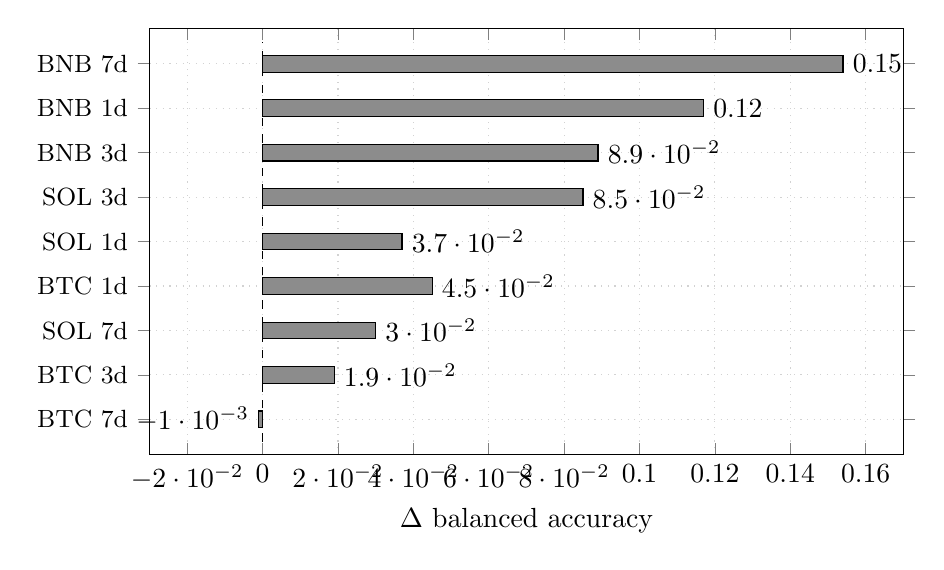
\begin{tikzpicture}
\begin{axis}[
    xbar,
    bar width=6pt,
    width=0.92\textwidth,
    height=7cm,
    xmin=-0.03,
    xmax=0.17,
    xlabel={$\Delta$ balanced accuracy},
    ytick={1,2,3,4,5,6,7,8,9},
    yticklabels={BTC 7d,BTC 3d,SOL 7d,BTC 1d,SOL 1d,SOL 3d,BNB 3d,BNB 1d,BNB 7d},
    yticklabel style={font=\small},
    nodes near coords,
    nodes near coords align={horizontal},
    grid=major,
    grid style={dotted,gray!35}
]
\addplot[fill=black!45, draw=black] coordinates {(-0.001,1) (0.019,2) (0.030,3) (0.045,4) (0.037,5) (0.085,6) (0.089,7) (0.117,8) (0.154,9)};
\draw[dashed] (axis cs:0,0.5) -- (axis cs:0,9.5);
\end{axis}
\end{tikzpicture}
\caption{Прирост balanced accuracy от добавления текстовых признаков относительно \texttt{market\_full} baseline}
\label{fig:run05_delta_balanced_accuracy}
\end{figure}

Наиболее выраженный эффект получен для BNB. На горизонте 1 день добавление FinBERT-derived и text-meta признаков к \texttt{market\_full} повышает balanced accuracy с 0.498 до 0.615, ROC-AUC --- с 0.476 до 0.670, а accuracy --- с 0.494 до 0.612. В отличие от случая, когда растёт только threshold-dependent метрика, здесь одновременно улучшается и ROC-AUC, то есть модель демонстрирует более высокую способность ранжировать наблюдения по вероятности положительного класса.

\begin{figure}[htbp]
\centering
\begin{tikzpicture}
\begin{axis}[
    ybar,
    bar width=12pt,
    width=0.78\textwidth,
    height=6cm,
    ymin=0,
    ymax=0.75,
    ylabel={Значение метрики},
    symbolic x coords={Accuracy,Balanced accuracy,ROC-AUC},
    xtick=data,
    x tick label style={font=\small},
    legend style={at={(0.5,-0.14)},anchor=north,legend columns=2},
    nodes near coords,
    nodes near coords align={vertical},
    grid=major,
    grid style={dotted,gray!35}
]
\addplot[fill=black!25, draw=black] coordinates {(Accuracy,0.494) (Balanced accuracy,0.498) (ROC-AUC,0.476)};
\addplot[fill=black!55, draw=black] coordinates {(Accuracy,0.612) (Balanced accuracy,0.615) (ROC-AUC,0.670)};
\legend{\texttt{market\_full},модель с текстовыми признаками}
\end{axis}
\end{tikzpicture}
\caption{BNB 1d: сравнение \texttt{market\_full} baseline и лучшей модели с текстовыми признаками}
\label{fig:run05_bnb_1d_market_vs_text}
\end{figure}

На горизонте 7 дней для BNB максимальный прирост balanced accuracy достигается у группы \texttt{text\_meta}: balanced accuracy увеличивается с 0.415 до 0.569, accuracy --- с 0.405 до 0.630, а ROC-AUC --- с 0.458 до 0.546. Это показывает, что часть новостного сигнала может проявляться не только на следующем дне, но и на более длинном горизонте. Однако лучший тип текстовой группы меняется между горизонтами: для 1d и 3d лучше работает комбинация рыночных признаков и FinBERT-derived признаков, тогда как для 7d наибольший прирост даёт более простая группа \texttt{text\_meta}.

Для BTC эффект положительный, но слабее. На горизонте 1 день balanced accuracy увеличивается с 0.457 до 0.503, а ROC-AUC --- с 0.473 до 0.483. На горизонте 3 дня balanced accuracy также немного растёт, но ROC-AUC снижается. На горизонте 7 дней добавочная сила текстов практически отсутствует. Следовательно, объём текстового корпуса сам по себе не является достаточным условием наличия прогнозного сигнала.

Для SOL текстовые признаки дают положительный прирост balanced accuracy на всех трёх горизонтах. На горизонте 3 дня balanced accuracy увеличивается с 0.516 до 0.602, однако accuracy снижается, а ROC-AUC растёт только незначительно. Поэтому результат по SOL следует интерпретировать как умеренно положительный, но менее устойчивый, чем результат по BNB.

Результат BNB следует рассматривать как кандидат на наличие текстового сигнала, а не как окончательное доказательство универсальной эффективности текстовых признаков. Итог RUN 05 отличается от RUN 04: если RUN 04 на AAPL не подтвердил добавочную силу FinBERT embeddings относительно расширенного рыночного baseline, то RUN 05 показывает, что на отдельных криптоактивах текстовые признаки могут давать существенный прирост. Следовательно, общий вывод работы должен быть условным: LLM/FinBERT-generated features не дают универсального преимущества, но могут быть полезны для отдельных активов, источников данных и горизонтов прогноза.
